% $Id: template.tex 11 2007-04-03 22:25:53Z jpeltier $

%\documentclass{vgtc}                          % final (conference style)
\documentclass[review]{vgtc}                 % review
%\documentclass[widereview]{vgtc}             % wide-spaced review
%\documentclass[preprint]{vgtc}               % preprint
%\documentclass[electronic]{vgtc}             % electronic version

%% Uncomment one of the lines above depending on where your paper is
%% in the conference process. ``review'' and ``widereview'' are for review
%% submission, ``preprint'' is for pre-publication, and the final version
%% doesn't use a specific qualifier. Further, ``electronic'' includes
%% hyperreferences for more convenient online viewing.

%% Please use one of the ``review'' options in combination with the
%% assigned online id (see below) ONLY if your paper uses a double blind
%% review process. Some conferences, like IEEE Vis and InfoVis, have NOT
%% in the past.

%% Figures should be in CMYK or Grey scale format, otherwise, colour
%% shifting may occur during the printing process.

%% These three lines bring in essential packages: ``mathptmx'' for Type 1
%% typefaces, ``graphicx'' for inclusion of EPS figures. and ``times''
%% for proper handling of the times font family.

\usepackage{mathptmx}
\usepackage{graphicx}
\usepackage{times}

%% We encourage the use of mathptmx for consistent usage of times font
%% throughout the proceedings. However, if you encounter conflicts
%% with other math-related packages, you may want to disable it.

%% If you are submitting a paper to a conference for review with a double
%% blind reviewing process, please replace the value ``0'' below with your
%% OnlineID. Otherwise, you may safely leave it at ``0''.
\onlineid{1636}

%% declare the category of your paper, only shown in review mode
\vgtccategory{Research}

%% allow for this line if you want the electronic option to work properly
\vgtcinsertpkg

%% In preprint mode you may define your own headline.
%\preprinttext{To appear in an IEEE VGTC sponsored conference.}

%% Paper title.

\title{Spot-Tracking Lens: A Zoomable User Interface for Animated Visualizations}

%% This is how authors are specified in the conference style

%% Author and Affiliation (single author).
%%\author{Roy G. Biv\thanks{e-mail: roy.g.biv@aol.com}}
%%\affiliation{\scriptsize Allied Widgets Research}

%% Author and Affiliation (multiple authors with single affiliations).
%%\author{Roy G. Biv\thanks{e-mail: roy.g.biv@aol.com} %
%%\and Ed Grimley\thanks{e-mail:ed.grimley@aol.com} %
%%\and Martha Stewart\thanks{e-mail:martha.stewart@marthastewart.com}}
%%\affiliation{\scriptsize Martha Stewart Enterprises \\ Microsoft Research}

%% Author and Affiliation (multiple authors with multiple affiliations)
\author{Yueqi Hu, Thomas Polk, Jing Yang, Ye Zhao, and Shixia Liu}
\authorfooter{
%% insert punctuation at end of each item
\item
 Yueqi Hu, Thomas Polk, and Jing Yang are with UNC Charlotte. E-mail: yhu12@uncc.edu.
\item
 Ye Zhao is with Kent State University. E-mail: zhao@cs.kent.edu.
\item
 Shixia Liu is with Tshinghua University. E-mail: shixia@tsinghua.edu.cn.
}

%% A teaser figure can be included as follows, but is not recommended since
%% the space is now taken up by a full width abstract.
%\teaser{
%  \includegraphics[width=1.5in]{sample.eps}
%  \caption{Lookit! Lookit!}
%}
%% Uncomment below to include a teaser figure.
   \teaser{
   \centering
   \includegraphics[width=18cm]{title}
   \caption{A screenshot of the spot-tracking lens. The lens is following Belarus in the year 1995. Ukraine and Tunisia are automatically labeled since they move faster than Belarus. The Slovak Republic and Russia are tracked. They are visible even when they go out of the spotlight.}
   \label{fig:title}
  }

%% Abstract section.
\abstract{Zoomable user interfaces are widely used in stationary visualizations and have many benefits. However, they are not well supported in animated visualizations due to problems such as moving objects, change blindness, and information overload. We propose the spot-tracking lens, a new zoomable user interface for animated visualizations and build a working prototype of it on animated bubble charts. It couples zooming with automatic panning and provides a rich set of auxiliary techniques to enhance its effectiveness. Our preliminary user studies suggested that, besides allowing users to examine detail information, it can be an engaging approach to exploratory analysis for dynamic data.} % end of abstract

%% ACM Computing Classification System (CCS).
%% See <http://www.acm.org/class/1998/> for details.
%% The ``\CCScat'' command takes four arguments.

\keywords{Animation; Zooming; Panning; Highlighting; Bubble Chart; Labeling}

% \CCScatlist{
%   \CCScat{K.6.1}{Management of Computing and Information Systems}%
% {Project and People Management}{Life Cycle};
%   \CCScat{K.7.m}{The Computing Profession}{Miscellaneous}{Ethics}
% }

%% Copyright space is enabled by default as required by guidelines.
%% It is disabled by the 'review' option or via the following command:
% \nocopyrightspace

%%%%%%%%%%%%%%%%%%%%%%%%%%%%%%%%%%%%%%%%%%%%%%%%%%%%%%%%%%%%%%%%
%%%%%%%%%%%%%%%%%%%%%% START OF THE PAPER %%%%%%%%%%%%%%%%%%%%%%
%%%%%%%%%%%%%%%%%%%%%%%%%%%%%%%%%%%%%%%%%%%%%%%%%%%%%%%%%%%%%%%%%
\begin{document}

%% The ``\maketitle'' command must be the first command after the
%% ``\begin{document}'' command. It prepares and prints the title block.

%% the only exception to this rule is the \firstsection command
\firstsection{Introduction}

\maketitle

%% \section{Introduction}

Zoomable user interfaces \cite{bederson1994pad,cockburn2008review,perlin1993pad} are widely used in information visualization systems. They allow users to magnify the view and thus see more details. Zooming brings many benefits to visualization: it allows users to examine the context of an interesting object by zooming in the area where the object resides; labels overcrowded in the original view can be displayed without overlaps after zooming in; it allows users to focus on a local area and thus reduce their cognitive load.

In spite of these benefits, zooming is not as well supported in animated visualizations as it is in stationary visualizations due to several challenges. First, objects are typically moving rather than staying still during an animation. Therefore, zooming has to be tightly coupled with panning for users to track objects of interest. Manual panning requires a lot of user effort to intensively follow moving objects, while automatic panning may cause difficulties for users to perceive the absolute speeds of objects in the view when the camera is moving unpredictably. In addition, users may lose their orientation with a frequently moving camera. Therefore, techniques helping users sense the absolute speeds of objects while maintaining orientation need to be developed to facilitate zooming coupled with automatic panning. Second, even after zooming in, multiple objects moving in varying speeds in the view can still cause huge cognitive loads on users.  Thus, the change blindness problem \cite{nowell_change_2001} can still prevent users from gaining insights from the data. Therefore,  auxiliary techniques based on the dynamic features of animation need to be developed to reduce change blindness to ensure users can enjoy the full benefits of zooming in an animated visualization.

In this paper, we present the spot-tracking lens, a new zoomable user interface specifically designed for animated visualizations (see Figure \ref{fig:title} for a screenshot). It couples zooming with automatic panning and provides a rich set of auxiliary techniques to help users sense object speeds, keep oriented, and reduce change blindness. In particular, the following techniques are explored in the spot-tracking lens:
\begin{itemize}
\item To support automatic panning, we propose two distinct view moving techniques. The stepwise panning technique simulates a user manually panning the view by dragging it; the continuous panning technique smoothly moves the view.
\item To help users sense the absolute speeds of the objects and keep oriented during panning, we propose to use a reference frame in the background of the animation and present an effective reference frame generation technique (see Figure \ref{fig:reference} for an example).
\item To reduce change blindness, we propose a novel spotlight technique to help users keep their attention focused on the immediate context of one object of interest, while still effectively tracking a few other objects of interest outside of this immediate context (see Figures \ref{fig:title} and \ref{fig:mask} for examples).
\item To reduce the cognitive load of users, we propose several task-oriented automatic labeling techniques that can direct user attention to the most important insights at any moment during the animation.
\item We propose to use scrolling to control animated visualizations. It allows users to seamlessly switch among automatic playing, stepwise  forward/backward, fast forward/backward, and pausing, and can thus improve the efficiency of analysis with animated visualizations.
\end{itemize}

\begin{figure}[t]
\centering
\includegraphics[width=\columnwidth]{reference}
\caption{The reference frame. Top row: screenshots of an animation segment showing a focal object moving up and to the right from 1953 to 1955. No reference frame is provided. Bottom row: screenshots of the same segment with a reference frame displayed. It is easier to sense the movement of the focal object in the bottom view. }
\label{fig:reference}
\end{figure}

\begin{figure}[!h]
\centering
\includegraphics[width=\columnwidth]{mask}
\caption{The spotlight. Left: A screenshot of a zoomed animation without using the spotlight. Right: The same scene with the spotlight turned on. Users are looking for fast moving objects, so only the focal object and its fast moving neighbors are labeled.}
\label{fig:mask}
\end{figure}

To illustrate the effectiveness of our ideas, we select the well-studied animated bubble chart as a representative animated visualization and develop a fully working prototype for it. Besides the expected benefits, our preliminary user studies revealed an unpredicted benefit of the spot-tracking lens: since it allows users to follow an object of interest for a long time without losing the focus and enables users to observe details, it greatly promotes ego-centric visual exploration, where the users gain a large number of inter-related, detail-rich insights around one or a few focal objects. Such long chains of insights are beneficial for sense making and reasoning. Therefore, this new technique may be useful in exploratory visual analytics of dynamic data.

\section{ Related Work}
\label{sec:relatedwork}
Animated visualization is an important approach to analyzing temporal data since human vision is sensitive to changes and movements. Hans Rosling presented the animated bubble chart (bubble chart for short) in his TED 2006 talk \cite{rosling_gapminder_2006}, where each bubble represented a country and its x position, y position, size, and color represented attributes of the country. The bubbles are animated to reveal changes in attributes over time. Rosling's talk invoked a lot of interest in animated visualization. Later, InfoCanvas \cite{miller_infocanvas:_2001} used moving entities to encode time series data. StreamIT \cite{alsakran2011streamit} used animation to illustrate the impact of newly arrived objects to the clustering structure of existing objects in streaming data. Visual Sedimentation \cite{huron2013visual} presented animated displays that imitated real-world sedimentation processes to represent data streams. GraphDiaries \cite{bach2014graphdiaries} used staged animations and complementary small multiples to help users understand changes between individual time stamps in dynamic networks.

However, recent studies reported that although animated visualization is fun and exciting \cite{farrugia2011effective,robertson_effectiveness_2008,tekusova_applying_2007}, it can be problematic in supporting analysis tasks. Robertson et al. \cite{robertson_effectiveness_2008} presented a user study comparing the bubble chart, small multiples, and traces for presenting and analyzing temporal data. The results showed that the bubble chart was the least effective in analysis, although it was rated as enjoyable and exciting. The authors pointed out that users can be confused by having too many data objects moving in the display. Farrugia and Quigley also pointed out that, when conducting analysis in animation, users can easily get lost when too many data objects are moving on the screen \cite{farrugia2011effective}. Clearly, a zoomable user interface can be a solution to this problem by allowing users to focus on a smaller set of data objects. However, existing applications, such as Gapminder (www.gapminder.org), are limited to stationary zooming, involving a labor-intensive process where users can only zoom into a fixed region and need to manually pan the view when the data objects of interest move out of the region.  We propose a new, zoomable user interface that tightly couples zooming and automatic panning.

Automatic panning has been studied in visualization. For example, Jark van Wijk et al. \cite {van2003smooth} discussed how to support smooth animations from one view to another by coupling panning and zooming. The speed-dependent automatic zooming \cite{igarashi2000speed} automatically changed the zoom level according to the panning speed. The spacetree application \cite{plaisant2002spacetree} automatically panned a view when users selected a different focal node in a tree visualization. Our approach uses automatic panning to track a moving focal area, which is a different scenario from the existing examples.

The complex manner of movement in animation may lead to change blindness \cite{french1953discrimination}, where users miss important temporal patterns \cite{nowell_change_2001,yi_toward_2007}. Change blindness can reduce the effectiveness of visual exploration even in a view that has been zoomed in. Many suggestions have been given in the literature on how to reduce change blindness in animation, such as ensuring that time intervals between different scenes are long enough, limiting the number of changes in animation through filtering and other interaction, and keeping users oriented with additional visual indicators \cite{schlienger2007improving}. Many of these ideas have been used in our design. For example, our approach allows users to flexibly control the animation speed, automatically labels the most important data objects at the current moment while suppressing the visual representations of the other objects, and provides a spotlight to allow users to follow the most interesting object and its immediate context.

In most animation systems, analysts control the animation by widgets such as buttons and sliders. Since these widgets are usually far away from the focal area, interacting with them interrupts users from watching the focal area. Archambault et al. \cite{archambault_animation_2011} found in a user study that subjects rarely used the play controls, even though using them could reduce the analysis time. Kondo and Collins \cite{kondo_dimpvis:_2014} attached a timeline to the trajectory of a focal object, making play control more tangible. However, this technique only applies to touch screens. We propose a different approach that is to use scrolling to control animation. Scrolling techniques have been used in story telling websites to control the speed \cite{frederick2013effects}. Our approach is among the first efforts to control animated visualization using scrolling.

\section{The Spot-Tracking Lens}
\label{sec:lens}
The spot-tracking lens is tied to a focal object rather than a selected region as in traditional approaches. To start the lens, a user selects a focal object and sets a zoom level. The new view will be magnified according to the zooming level and keep the focal object in the view. During the animation, the camera roughly follows the movement of the focal object with automatic panning. In the following sections, we present the automatic panning and other auxiliary techniques used in the spot-tracking lens.

\subsection {Automatic Panning}
Three different automatic panning strategies have been explored. In the first approach, the focal object is always centered in the view. Therefore, it is easy for users to observe the relative movement of the other objects with regard to the focal object. However, whenever there are noises in the track of the focal object, users would incorrectly perceive that the tracks of all the other objects are noisy. In addition, it is difficult for users to sense the movement of the focal object with this approach. Therefore, we propose two other panning methods. Stepwise panning simulates manual panning and continuous panning smoothly follows the focal object without jitter. Each algorithm consists of two steps: (1) determining a sequence of view center positions in the global view according to the trajectory of the focal object and (2) determining the starting time and end time for the view center to move from one position to the next during the animation. The transition between the two positions is created by interpolation.

{\bf Stepwise Panning}: The idea is to pan the view when the focal object is about to run out of the view. This is a strategy often used by human beings when conducting manual panning. This method only pans the view when necessary, thus reducing the additional cognitive load imposed by panning. An algorithm is proposed to determine the view center positions (see Figure \ref{fig:stage} A): Creating a sequence of bounding boxes, each having the same size as the view, to cover all the focal object positions along its trajectory. The centers of the bounding boxes are the view center positions along the sequence. To allow users to examine the context of the focal object, the bounding boxes can be set to be smaller than the view (see Figure \ref{fig:stage} B), to ensure a minimum distance between the focal object and the view boundary.

\begin{figure}[t]
\centering
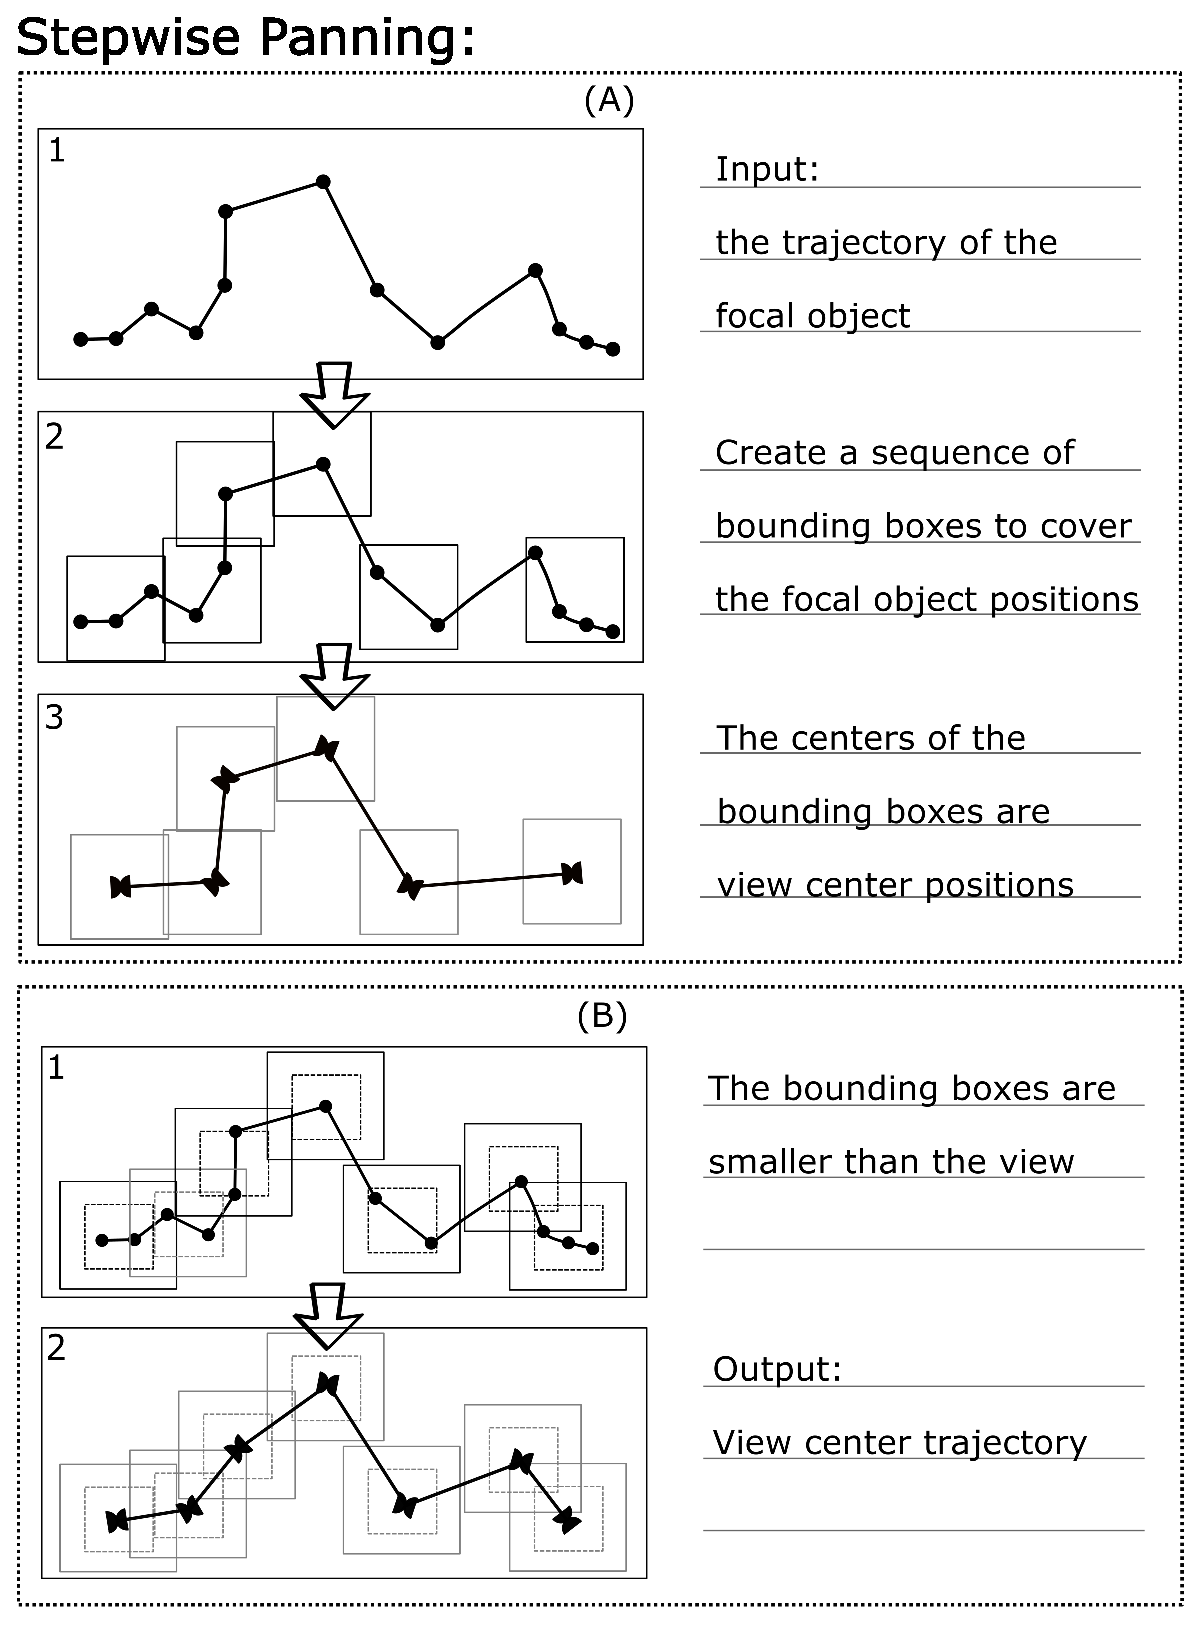
\includegraphics[width=\columnwidth]{stage}
\caption{Illustration of view center trajectory generation for stepwise panning.}
\label{fig:stage}
\end{figure}

When a user zooms in at any moment during the animation, the view center is first set to be the center of the bounding box covering the current focal object position. If the next position of the focal object is within the same bounding box, no panning will be triggered. Otherwise the view center moves to its next position, starting at the same time when the focal object starts moving and finishing when the focal object reaches its next position. In stepwise panning the focal object is not always close to the view center. It also creates an illusion of steps in focal object's movement. Continuous panning overcomes these problems by moving along a smooth trajectory with evenly distributed steps.

\begin{figure}[t]
\centering
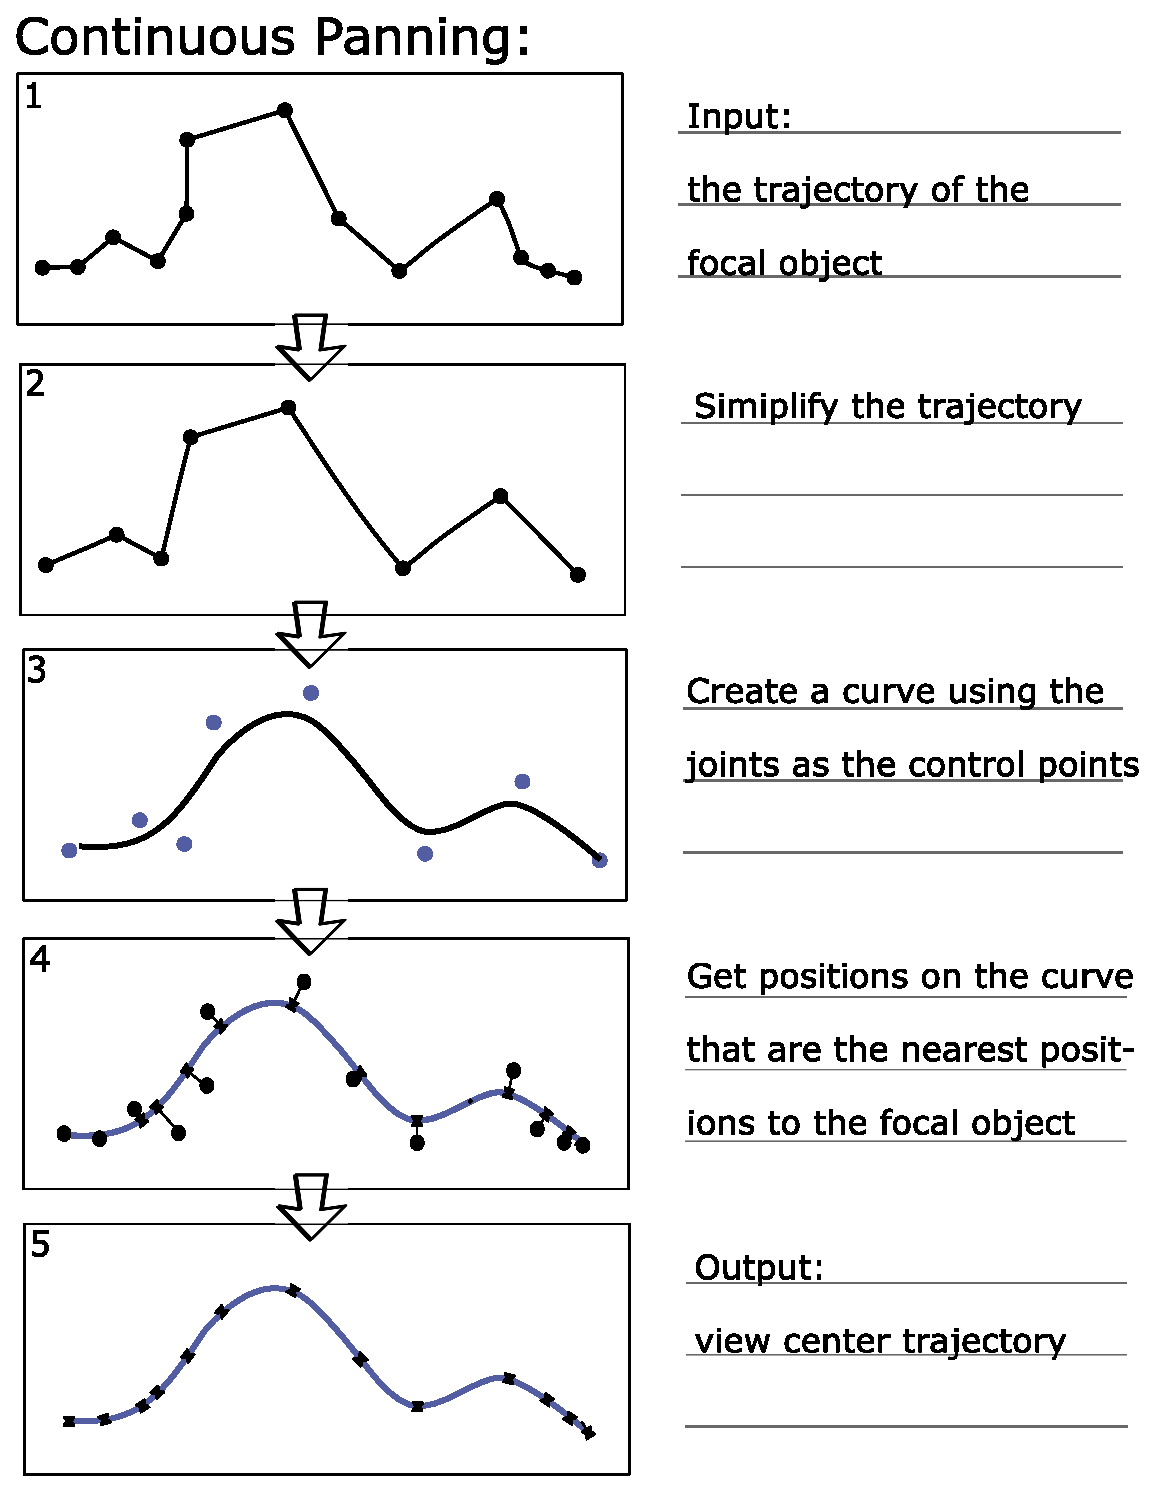
\includegraphics[width=\columnwidth]{follow2}
\caption{Illustration of view center trajectory generation for continuous panning.}
\label{fig:follow2}
\end{figure}

{\bf Continuous panning}: Continuous panning follows the focal object in a smooth long shot, similar to the way a camera follows a runner running in a race. Figure \ref{fig:follow2} illustrates our algorithm for determining the view center positions: First, the focal object trajectory is simplified to a trajectory with less joints using the Douglas–Peucker algorithm \cite{heckbert1997survey}. The tolerance threshold in the Douglas–Peucker algorithm is set to different values for different zoom-in factors, so that the simplified trajectory preserves more details when the camera is closer to the focal object. Second, joints in the simplified trajectory are used as control points to create a Bezier curve \cite{yamaguchi1988curves}. Third, for each focal object position, we calculate its closest point on the curve. These points are the view center positions. To avoid jitters, the order of view centers on the curve should be the same as the order of focal object positions. Whenever the focal object moves to a new position, the view center also moves to the corresponding nearest point on the curve. In this way, the focal object is usually close to the view center and the panning is smoothed.

\subsection{Reference Frame}
When automatic panning is used, users may have difficulties in judging how the objects are moving. We introduce a reference frame to address this problem. When we sit in a train, we feel it is moving forward because the landscape outside the window is moving backward. Here, the landscape plays a role as the {\bf frame of reference}. Similar frames of reference are developed in the spot-tracking lens. They are static background in the global view, thus users can sense the movements of objects in the global view by watching how the objects move related to a reference frame. Textured images, grids, and other images can be used as reference frames. No matter what they are, they should be unattractive and non-distracting to avoid adding additional cognitive load to users. In our prototype, we use the combination of the silhouette of the focal object trajectory and an optional background texture as the reference frame (see Figure \ref{fig:title}).

The silhouette is cleaner and less distracting than the trajectory and more informative than backgrounds such as grids. It is created using the following algorithm: starting from N = 1, we create a convex hull to cover all the positions numbered from N to N+M along the focal object trajectory (where M is a positive integer). A smaller M preserves more details of the trajectory variation, which is preferred when the zoom level is large. This process is repeated by increasing N until all the points on the trajectory are covered. Then, we combine all the convex hulls to form the trajectory silhouette. The shape of the silhouette shows the temporal trend of the focal object. A stable focal object movement creates slim and smooth silhouette. Such information can help users predict the motion behavior of the focal object. Finally, we set the silhouette to be semi-transparent, which makes it easy to observe but not distracting. In addition, a plane symmetry group background texture (see the round things  in the background of Figure \ref{fig:title}) is used to fill the background.

\subsection{The Spotlight}
In stage arts, a spotlight is often shed on a focal character and moves synchronously with her. The characters in the dark do not attract attention unless they get close to the focal character. The spotlight follows the focal character to illustrate an ego-centric story around her: at times, other characters run into the spotlight to meet her or she approaches and leaves other characters. A similar technique is used in the spot-tracking lens. As shown in Figure \ref{fig:mask}, the spotlight is always centered on the focal object, highlighting its immediate context as a focal area. During the animation, the spotlight moves synchronously with the focal object, magnifying its  movements (the spotlight is much larger than the focal object), attracting user attention to itself and its context, and allowing users to examine details in the focal area.

There are two ways to get attention: let the focus be more attractive, or let everything else be less attractive. Both strategies are used in the spotlight. To make the focal object more attractive, it is highlighted by a time stamp displayed above it. To make objects far away from the focal object less attractive, the area outside of the spotlight is covered by a semi-transparent dark gray mask. Not only masked, the objects in this area are changed from varying sized colorful circles to small, dark circles, which are not attractive in the dark gray background. Their labels are also turned off. In addition, a light gray middle tone area provides a transition between the spotlight area and its surrounding context. Outside the middle tone, a thin darker shadow area enhances the spotlight's boundary. It also indicates the boundary of the region where the objects are readable with their original labels, sizes, and colors. We slightly decorates the shadow using the hue of the focal object. The size of the spotlight can be interactively adjusted by users. Users can also turn the spotlight or its subareas on or off.

The assumption underlying the spotlight design is that objects outside of the focal area are unimportant since they are far away from the focal object. However, in the dynamic environment, an object can be close to the focal object in one moment and far away in the next. In this situation, users may keep a long term interest in it. For example, they may want to check if the object comes close to the focal object again or compare the overall movement of the object with that of the focal object in a longer time sequence. To support this need, a tracking interaction is provided where users can click an object in the view to highlight it. Highlighted objects are always displayed with labels and are never degraded and masked. Therefore, they are easily seen in the dark gray background when they move out of the focal area (see Figure \ref{fig:title} for an example).

\subsection{Selective Labeling}
Labels provide important semantic information in visualizations \cite{fekete1999excentric}. In animated visualizations, manual labeling approaches may require intensive human efforts since insights and relevant objects may change over time. The ``label all'' strategy may causes clutter even in a magnified view. We propose a new labeling strategy called selective labeling. It automatically labels and de-labels objects of interest and objects that are no longer of interest during the animation based on pre-defined user tasks.

The implementation of the selective labeling can be as simple as: (1) at each moment, calculate an importance value for each object in the view and rank the objects in the view from high to low; (2) label the top N objects (N is set by users to show more or fewer labels); if a labeled object is no longer in the top N, turn off its label. However, this simple algorithm causes a problem. Since the ranking directly reflects the dynamic importance of the objects that may change frequently, the objects repeatedly entering and leaving the top N list show as twinkling labels. Twinkling labels are not desired since they distract users from examining labeled objects. We explored several ideas for anti-twinkling.

The first idea is to make the ranking more stable. To do so, the importance values of the objects are calculated in a sliding time window centered at the current time stamp. This approach reduces the twinkling but cannot guarantee to eliminate the effect completely. The second idea is a heuristic anti-twinkling technique. A label should not be removed (if the object is still in the display) for at least M (M is 3 in the current prototype) consecutive time steps. Therefore, if an object is dropped from the top N and soon comes back, its label will be kept on during the gap. The two ideas are used together in our prototype and effectively reduce twinkling.

We now present how to automatically label objects that are the nearest to the focal object. Note that we can observe objects passing by the focal object during their movement. Users often consider them as close to the objects and want to identify them. It is different from stationary visualization where only static positions need to be considered. We propose the following algorithm to determine the importance values of objects according to such closeness:

Considering two objects p and s, whose locations at time step 1 are $s_{1}$, $p_{1}$ and whose locations at time step 2 are $s_{2}$ and $p_{2}$, we interpolate their moving path between the two time steps. The minimum distance between them can then be computed as
\begin{equation}
\min_{d \in [0,1]}  \parallel  (\overrightarrow{p_1}*d+ \overrightarrow{p_2}*(1-d) )-(
\overrightarrow{s_1}*d+ \overrightarrow{s_2}*(1-d)) \parallel
 \end{equation}
where $d$ ($0<d<1$) is the time between the two steps. The average minimum distance between an object and the focal object in the time window is the importance value to be used in the selective labeling algorithm.

The importance value can be defined in different ways to support different tasks. For example, using the moving speeds of the objects as the importance values can capture objects that are moving fast. They are changing dramatically and are thus worth the attention of users. Since a time window is used, an object can be labeled prior to a fast movement and therefore help users capture volatile patterns.

\subsection{Scrolling}
Unlike watching a movie, exploratory analyses require full control of time and playing speeds. As Kondo and Collins suggested \cite{kondo_dimpvis:_2014}, animated visualization should allow users to directly interact with the scene to manipulate the animation. In addition, it is difficult to display a timeline which is long enough for precise speed and time control. Therefore, instead of using a visible timeline, the spot-tracking lens is implemented in a webpage and uses scrolling to control a virtual timeline of the animation, inspired by the parallax scrolling websites \cite{frederick2013effects}. Users can scroll the mouse wheel to control the animation, as if they were browsing a long webpage. Scrolling position decides which time frame of the animation to show. Most control functions can be conducted through the mouse wheel: users can scroll up or down to play backward or forward as well as drag the scroll bar to jump to a certain position of the timeline. The users keep scrolling to make the animation continue or pause scrolling to pause the animation for detail examination. They can control the animation speed by changing the scrolling speed, which is much easier than using a speed control slider. Users can easily change the speed without the penalty of being interrupted by switching their attention to adjust a slider.   To encourage users to scroll slowly, we disable transitional animation between frames when the scroll speed is beyond a threshold. In other words, users will see key frames flashing one by one like a video played in fast forward mode when they scroll quickly. It is an ideal play control for users to change the animation speed frequently or pause the animation from time to time for detail analysis. Users can also start an auto-play mode by clicking a button and switch back to manual speed control at any time by scrolling the mouse wheel.

\section{Spotlight User Study}
\label{sec:spotlightstudy}
A user study was conducted to evaluate the following hypotheses: (1) The spotlight can help users focus on a focal area moving around in the view. (2) The spotlight can help users track a moving focus area when there are objects moving in its surrounding area. (3) The spotlight can help users track a small set of highlighted objects while paying attention to a moving focal area, especially when they are not in the focal area.

A subset of a world wealth and health dataset downloaded from Gapminder \cite{rosling_gapminder_2006} was used in this study. It contains data about 200 countries since 1900. The populations of the countries were mapped to the bubble size. Life expectancies were mapped to the y axis and average income was mapped to the x axis. Countries are grouped into 6 geographical regions: Asia and Pacific, Sub-Saharan Africa, Middle East and North Africa, South Asia, America, Europe and Central Asia. The regions were represented by the color of the bubbles.

Twenty subjects (10 males and 10 females) participated in this study one-by-one. They were graduate students majoring in Computer Science. All of them were taking a graduate level Information Visualization class. They learned about animated bubble charts, zooming, panning, and labeling before the user studies.

Five pairs of videos were presented to each subject side-by-side in a web browser. Each video lasted about 30 seconds. Each pair of videos consisted of the same segment of animation of a zoomed, animated bubble chart with the spotlight turned on or off. In all the videos, the focal object was highlighted by a thin, yellow halo, so it was slightly different from other objects in the view. Two pairs of videos were created for evaluating the first hypothesis: the ``move'' videos show a focus region moving in the view; the ``fixed'' videos show a focus region fixed in the center of the display during the animation. Two pairs of videos were created for evaluating the second hypothesis: the ``cluttered'' videos show a moving focal area with a lot of objects moving in the area outside; the ``sparse'' videos show a moving focal area with only a few objects moving in the area outside. The ``multi-tracking'' videos evaluated the third hypothesis. They show five objects highlighted by thin yellow halos moving around in the view. They are not darkened by the masked area outside of the spotlight at any time. In all the videos, all the bubbles are colored and labeled and have varying sizes.

When a subject opened the web browser, a video pair was displayed in the web browser. The user clicked a play button to watch a video. When watching the multi-tracking videos, users were asked to track the highlighted objects while paying attention to the moving focal area. When watching the other videos, users were asked to speak out the name (or the first letter) of the country closest to the focal country in every year. The subject watched the two videos in random order. After watching the videos, users selected the preferred video or indicated no difference through a check box. Users then clicked a button to watch the next pair of videos. The video pairs were randomly ordered for each subject. Study results are shown in Figure \ref{fig:spotlightstudy}.

\begin{figure}[t]
\centering
\includegraphics[width=\columnwidth]{spotlight}
\caption{Videos preferred in the spotlight user study.}
\label{fig:spotlightstudy}
\end{figure}

\begin{figure*}[htb]
 \centering
 \includegraphics[width=1\linewidth]{Germany}
\vspace{-0.2in}
 \caption{The journey of Germany after World War II. 1: Germany recovers from WWII in 1945 quickly. 2 and 3. Germany quickly surpasses other European countries such as France and Belgium. 4. In 1967, Japan moves forward to join Germany's neighborhood. 5. More red bubbles (Asian countries) join Germany's neighborhood in 1989. Meanwhile, Germany retreats a little bit as the result of reunification. 6. Red bubbles continue their progress in surpassing Germany.}
 \label{fig:germany}
\vspace{-0.21in}
\end{figure*}

\begin{figure*}[htb]
 \centering
 \includegraphics[width=1\linewidth]{India}
\vspace{-0.2in}
 \caption{The journey of India around its independence. 1, 2, and 3. Asian countries such as China, Vietnam, the Philippines, and Indonesia are in an unstable status as they are involved in World War II. India is relatively stable. 4, 5, and 6. In 1946, countries like Vietnam are recovering from the War. India, on the contrary, drops slightly but soon recovers by 1948. Meanwhile, Pakistan also drops and recovers synchronously.}
 \label{fig:india}
\vspace{-0.21in}
\end{figure*}

From the results we can see that more subjects preferred the animation with the spotlight on than without it off in all the scenes, especially when multiple objects needed to be tracked while following a focal area at the same time (confirming all the three hypotheses). The subjects commented that it was much easier to see the bright bubbles on a dark background. More subjects preferred the spotlight when the focal area was moving around than when it was fixed. The spotlight was less preferred when more distractors were moving in the area outside of the focal area, which suggests that an upper limit of objects that can be tracked at the same time should be limited in the spotlight.

\section{Open-Ended User Study}
\label{sec:casestudy}

In this preliminary user study, we investigated how the spot-tracking lens changed the subjects' visual exploration strategies and the types of insights they captured in exploratory analysis. We also recorded several cases generated by the subjects to illustrate the utility of this zoomable user interface. Two systems were used in this study: one was the animated bubble chart provided from Gapminder (Gapminder for short) \cite{rosling_gapminder_2006}; the other was the zoomable user interface we developed on the animated bubble chart (SpotLens for short). We wondered whether SpotLens could provide an alternative perspective in the exploration of time series data.

Two groups of subjects participated in this study. Each group consisted of two master students with visualization background who were familiar with each other; they were asked to work together to explore world history after 1900 using the systems. They spent one hour on each system, with a break of at least one hour between the two sessions. The two sessions were conducted in the same day. One group used Gapminder first and the other used the SpotLens first. The instructor trained the subjects on how to use the system before each session. She observed all the sessions and video recorded them. The subjects were told that insights about the relationships among multiple countries were more valuable than insights about single countries, since the latter can be easily captured by static displays.

First, we present two stories captured by the subjects.

{\bf The story around Germany}: Subject group A investigated the dataset by setting Germany as the focal object (see Figure \ref{fig:germany}). They turned on the selective labeling to highlight countries close to Germany and ran the animation starting from World War II. They found that after World War II, Germany surpassed many western European countries in both X and Y axes within a 20 year period. Figure \ref{fig:germany} shows a snapshot of the animation after Germany surpassed France and Belgium. After this time period, Germany maintained its rapid progress and surpassed the United Kingdom. Then, the subjects noticed that Japan came into the race and joined Germany's neighborhood. They noticed that Japan had been the only Asian country (red bubble) in this neighborhood until 1980, when many more red bubbles appeared in the neighborhood (see Figure \ref{fig:germany}). They argued that Asia had its biggest leap at that time according to this observation.

{\bf The story around India}:Subject group B selected India as the focal object (see Figure \ref{fig:india}) and enabled automatic labeling for fast moving objects. In the zoomed view they were able to read the names of fast moving countries in India's neighborhood. They saw countries such as China and Vietnam during World War II. These names made sense to them since they were the World War II participants. After World War II, they were surprised to see that India experienced a slight drop in 1946 while most other countries around it were quickly recovering from the war. They also noticed that Pakistan had a similar experience. They suspected that it might be relevant to the Partition of India and Pakistan in 1947.

We now discuss the observations from the study:
\begin{itemize}
\item Leaps: Gapminder users captured large leaps of big countries easily. They also captured several small countries when they were leaping to a sparse area, but they did not notice leaps occurring in cluttered areas. SpotLens users captured leaping countries when they were in the view, even in cluttered areas. They were able to capture small leaps such as the one mentioned in the India story. Such leaps are not noticeable in either Gapminder or static displays.
\item Inter-country relationships: It was noticed that subjects observed many more inter-country relationship insights in SpotLens. With Gapminder, the comparison often relied on the subjects' pre-knowledge of a country's history. The subjects had to add trails for two countries to examine their relationships.
\item Maintaining attention: As shown in the Germany story, SpotLens users were able to keep their interest in a country longer and discover many insights about it. It was also observed that the subjects jumped to a focal object after finding interesting insights about it when exploring another focal object. The exploration patterns in Gapminder were quite different. The subjects more often followed the mode of generating a hypothesis based on pre-knowledge - verifying the hypothesis using animation - and then generating another hypothesis based on other pre-knowledge. The difference suggested that SpotLens may be a useful technique for ego-centric visual explorations and progressive visual explorations.
\end{itemize}

The leap discovery observation confirmed that SpotLens helps users examine fine details during animation as expected. We did not anticipate the advantages SpotLens provides in finding inter-country relationships and supporting ego-centric and progressive visual explorations. It hints that SpotLens may be an engaging and inspiring approach in exploratory analysis of dynamic data, which needs to be investigated in future user studies.

After the subjects finished both sections, preferences and feedback were collected from them. All subjects agreed that SpotLens and Gapminder were designed for different tasks and they should work together to get more insights. The subjects all gave positive feedback to the visualization design of SpotLens. They commented that its trajectory silhouette background looked good and was informative; they could read labels easily in SpotLens; its design was artistic; and it was flexible to go back and forth and control speed through scrolling in SpotLens.

\section{Conclusion}
\label{sec:conclusion}

In this paper, we propose the spot-tracking lens, a new zoomable user interface for animated visualizations and present its fully working prototype on animated bubble charts. It not only allows users to enjoy the expected benefits of zooming, such as focusing on focal objects and their context, examining details and labels in a less cluttered view, but also brings additional benefits into animated visualization. Our preliminary user study suggested that it can be an engaging user interface for ego-centric, progressive visual exploration of dynamic data. Our exploration also reveals that interactions, such as zooming, face new challenges in animated visualization that are not encountered in traditional stationary visualization. It is an under-explored research area where new efforts can be challenging yet productive. We argue that new techniques developed in this area may help solve the dilemma that animated visualization is fun and exciting, but less effective than stationary visualization in supporting analysis tasks. After a complete set of interactions are developed in the future, animated visualization may fully reveal its effectiveness and efficiency in analysis tasks.

The main contributions of this paper are:

\begin{itemize}
\item We present a new zoomable user interface for animated visualization. It couples zooming with automatic panning, and provides a set of auxiliary techniques, such as reference frames, spotlight, and selective labeling, to address problems such as change blindness, orientation maintenance, and clutter.
\item We implemented a fully working prototype of the zoomable user interface for animated bubble charts. Our preliminary user studies suggested the benefits of the interface in encouraging ego-centric, exploratory visual analytics, besides the zooming benefits seen in stationary visualizations.
\end{itemize}

In the future, we will develop other interactions for animated visualization, such as distortion techniques and dimension management techniques, and investigate how they improve the effectiveness of animated visualization for visual analytics. We will also test how our zoomable user interface works on animated visualization other than bubble charts and further analyze how it promotes exploratory visual analytics.

%% if specified like this the section will be committed in review mode

\bibliographystyle{abbrv}
%%use following if all content of bibtex file should be shown
%\nocite{*}
\bibliography{template}
\end{document}

%%% Local Variables:
%%% mode: latex
%%% TeX-master: t
%%% End:
